\chapter{Dataset}
\label{ch3}
Data preprocessing is an essential step in producing an effective machine learning model. The data for training must be representative of the problem being modeled, and the validation and test sets should be representative of the train dataset. Failing to satisfy these conditions can lead to an ineffective model, validation results that lead to poor model and hyperparameter selection, and testing results that inaccurately represent a model's capability. This Chapter steps through the preprocessing applied to the $C_{n}^{2}$ and weather data including filtering, window averaging, formatting into input sequences and forecasts, and parsing into train, validation, and test datasets.

\section{Measurement Collection Setup}

\subsection{Weather Measurements}
The entire dataset uses time correlated weather and $C_{n}^{2}$ measurements. The weather measurements are from a Davis Instruments Vantage Pro2 Plus weather station \cite{davis} deployed in front of an office building from 12 April 2020 through 10 August 2020. The weather variables recorded by the station and considered in this work are temperature, pressure, relative humidity, wind speed, and solar irradiance. Table \ref{tab:weather_station} lists the technical specs of the weather station including the measurement resolution, accuracy, and archive interval.
\begin{table}[h!]
	\begin{center}
		\caption{Davis Instruments Vantage Pro2 Plus Weather Station Measurements \cite{davis}}
		\label{tab:weather_station}
		\begin{tabular}{||l|c|c|c||}
			\hline
			Variable & Resolution & Accuracy $\pm$ & Archive Interval \\
			\hline
			\hline
			Temperature & 0.1\textdegree C & 0.3\textdegree C & 1 min \\
			\hline
			Pressure & 0.1 mb & 1.0 mb & 1 min \\
			\hline
			Relative Humidity & 1\% & 2\% & 1 min \\
			\hline
			Wind Speed & 0.45 m/s & 5\% & 1 min \\
			\hline
			Solar Irradiance & 1 $W/m^{2}$ & 5\% & 1 min \\
			\hline
		\end{tabular}
	\end{center}
\end{table}

The variable resolution refers to the minimum difference measurable, for example relative humidity can distinguish between 90\% and 91\%, but not between 90\% and 90.5\%. The resolution of wind speed, 0.45 m/s, is 1 mph (mile per hour) resolution converted to m/s. Variable accuracy is the variable error per measurement, so for example a measurement of relative humidity of 90\% is has an error range of $\pm$ 2\%. Finally, the archive interval indicates how often the variable is reported. The archive interval is different from the measurement frequency. The anemometer measures wind speed every 2.5 to 3 seconds but the average over the archive interval, 1 minute, is reported. The archive interval of this dataset is 1 minute, the shortest interval available from the weather station.

The location of the weather station is on a storm drain surrounded by grass, about 20 feet to the southwest of a single-story office building. The weather station is not obscured by any trees or shrubbery in very close proximity. To the south of the weather station about 180\textdegree field of view is completely open space. The wind measurements are taken by an anemometer about 3 meters above ground level (AGL). The other measurements are recorded about 2.5 meters AGL. Figure \ref{fig:setup_weather} illustrates the location of the weather station and labels the key sensors and solar panel. The image in Figure \ref{fig:setup_weather} is taken from the southeast to illustrate the proximity of the station to surrounding geography to the northwest. To the right of the image is the office building about 20 feet away.
\begin{figure}[h!]
	\centering
	\includegraphics[width=0.65\textwidth]
	{setup_wx_station.png}
	\caption{Weather station deployment}
	\label{fig:setup_weather}
\end{figure}

\subsection{Turbulence ($C_{n}^{2}$) Measurements}
\label{sec:summary_tub_meas}
The other component of the dataset is minute-by-minute measurements of $C_{n}^{2}$ as measured by an MZA DELTA (\underline{Del}ayed \underline{T}ilt \underline{A}nisoplanatism) turbulence profiler. The DELTA is a passive imaging sensor that uses a monochrome camera attached to a 6-inch telescope with 1.5 m focal length. The DELTA calculates differential jitter as a function of angular separation to measure $C_{n}^{2}$ by collecting 300 frames (images) of a target of opportunity at 100 Hz. It's desirable for the target to have  high contrast features like edges and corners throughout the image to make measurements of differential jitter at variety of separations. Separations of 0.5 to 20 aperture diameters are recommended, so for a 6" telescope aperture the smallest feature separation would be 3" and largest 10' apart in the target plane.

The $C_{n}^{2}$ measurements in this work span from 12 April 2020 through 10 August 2020. During this time the DELTA was deployed on the 5th floor of Fitz Hall at University of Dayton in Dayton, Ohio. Figure \ref{fig:setup_DELTA_a} is a picture of the DELTA's deployment in Fitz Hall.
\begin{figure}[p!]
	\centering
	\subfloat[Telescope setup\label{fig:setup_DELTA_a}]{
		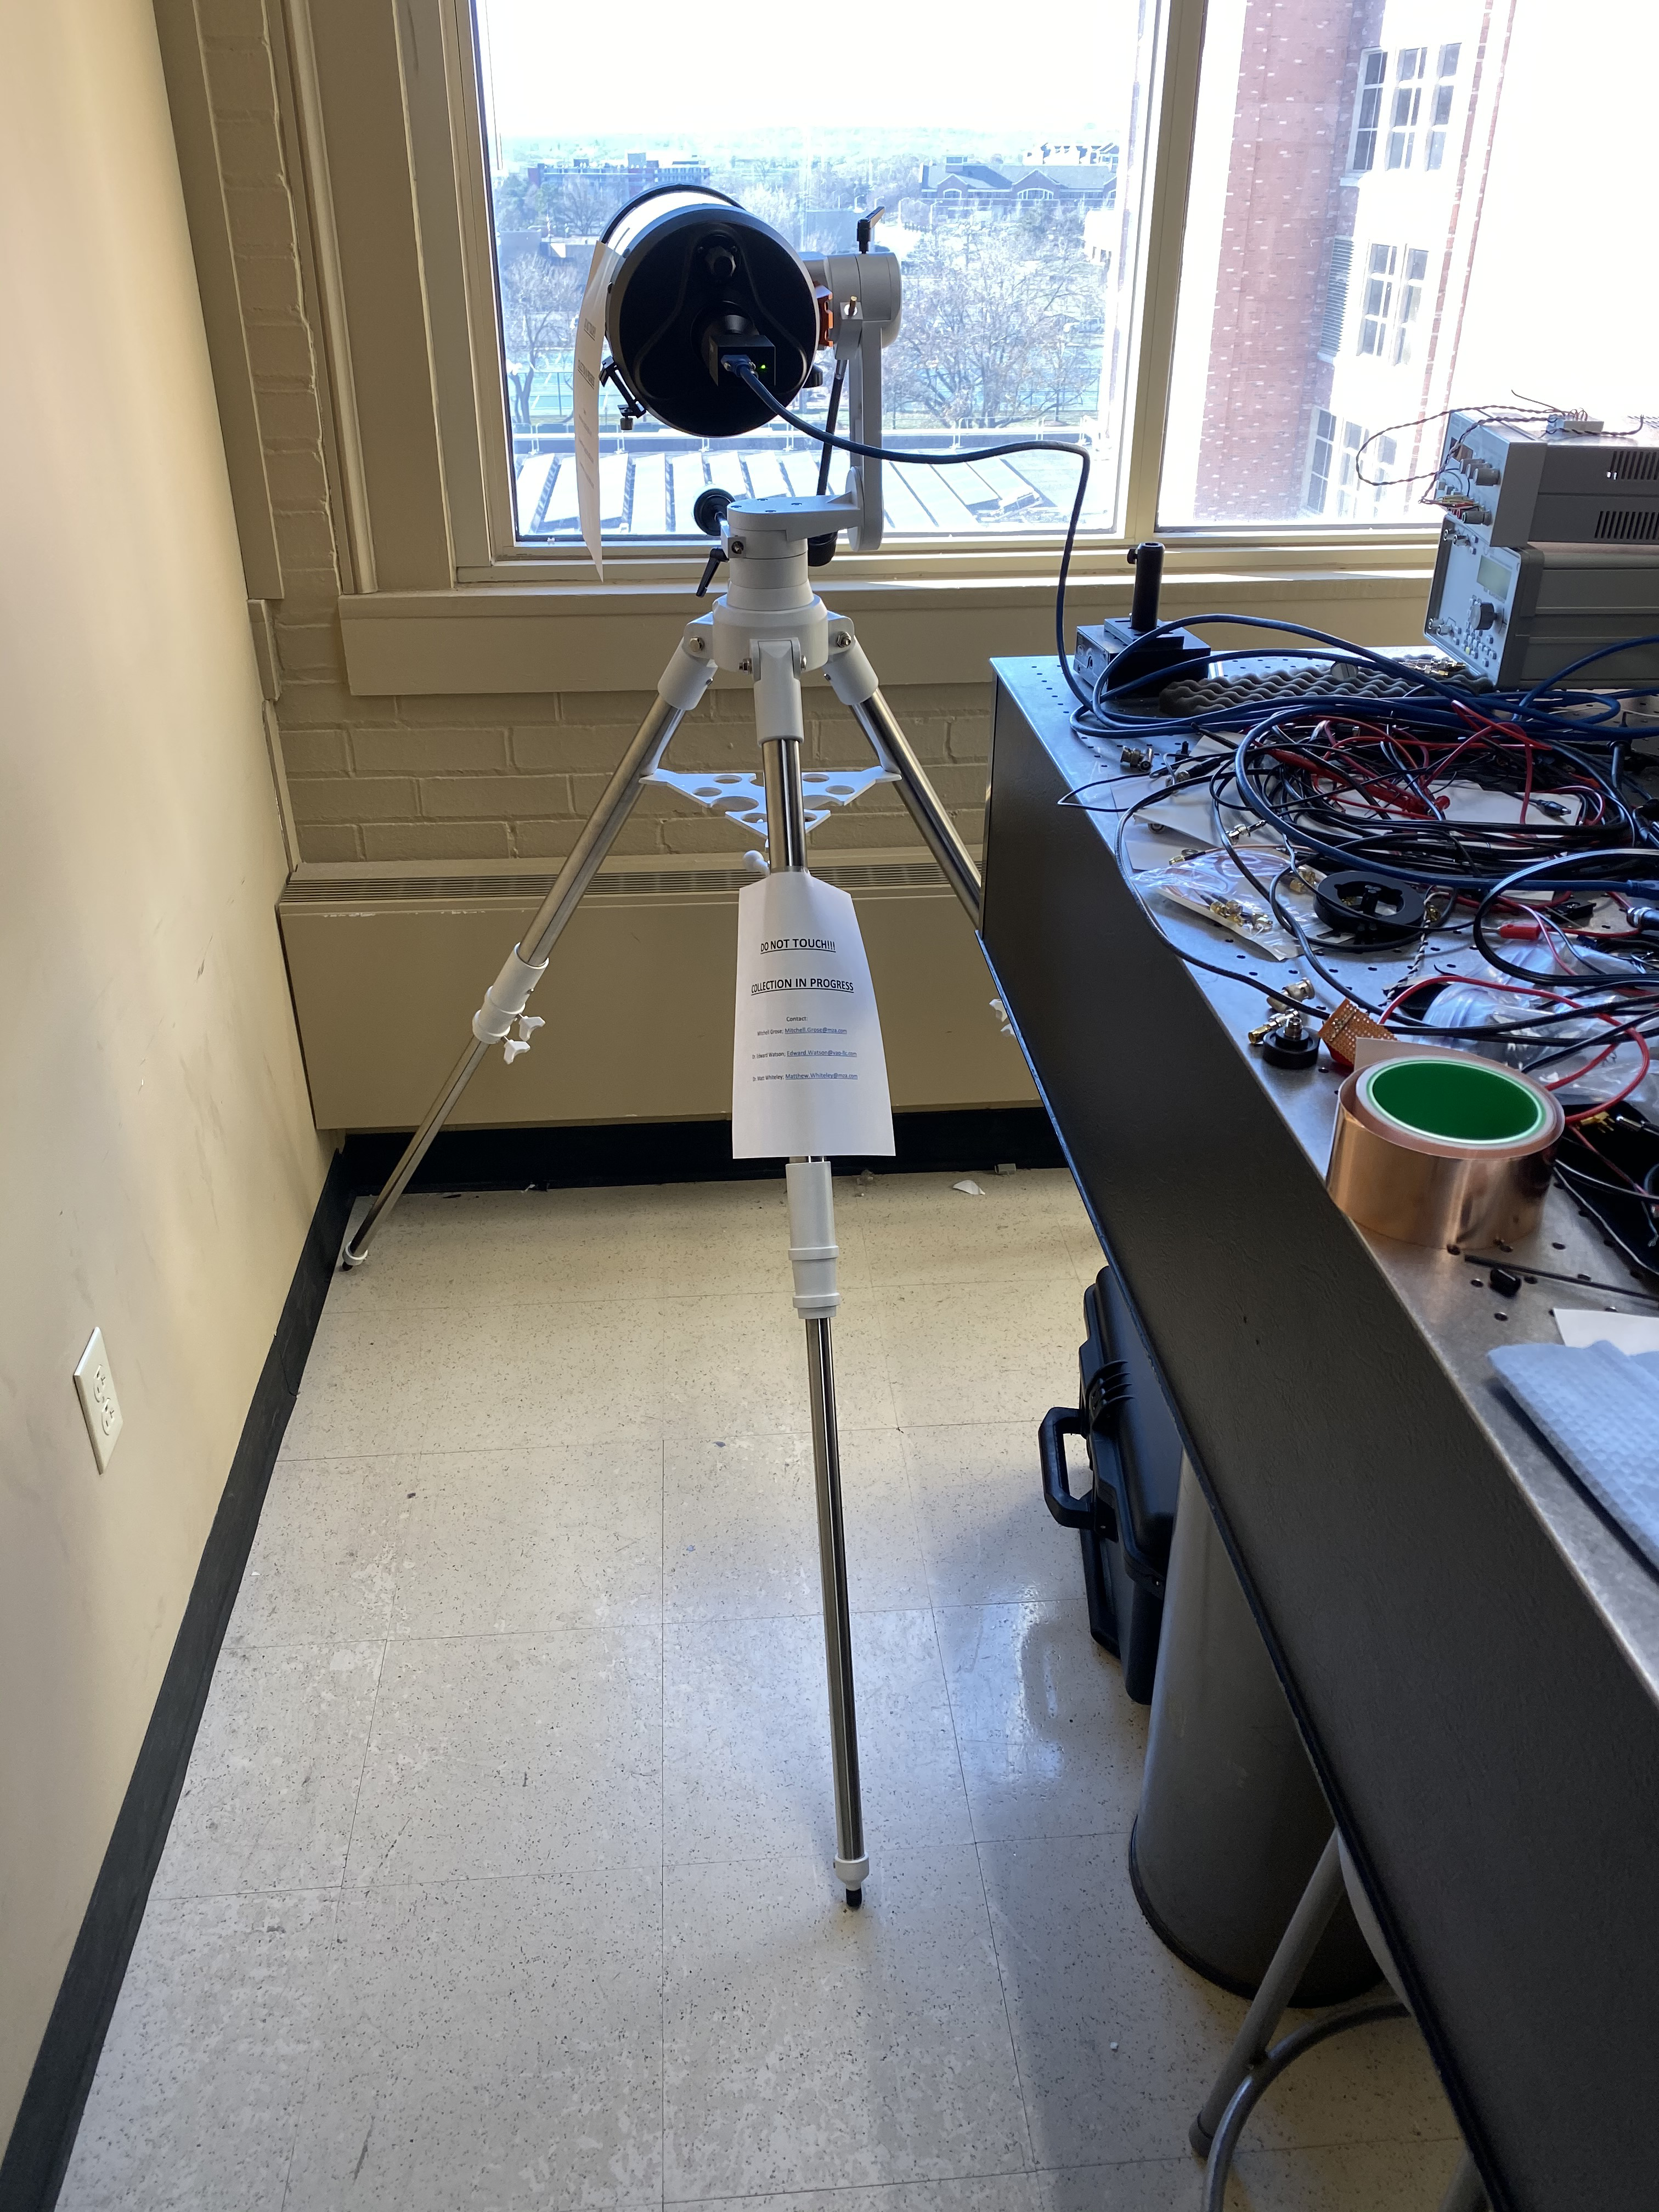
\includegraphics[width=0.49\textwidth]
		{DELTA_setup1.png}
	}
	\subfloat[Wide view of target\label{fig:setup_DELTA_b}]{
		\includegraphics[width=0.49\textwidth]
		{DELTA_setup3.png}
	}
	\hfill
	\subfloat[Narrow view of the target\label{fig:setup_DELTA_c}]{
		\includegraphics[width=0.49\textwidth]
		{Y_Tower.png}
	}
	\subfloat[Target as seen by the DELTA\label{fig:setup_DELTA_d}]{
		\includegraphics[width=0.49\textwidth]
		{FirstFrame_LowTurb.png}
	}
	\hfill
	\caption{DELTA setup for and target view for collection of minute-by-minute $C_{n}^{2}$ measurements.}
	\label{fig:setup_DELTA}
\end{figure}
The target the DELTA observes throughout the collection is the \textit{WRGT/WKEF TV Dayton} tower to the southwest of the sensor. The range to the target is 6.4km. The platform is approximately 249 meters above mean sea level (AMSL), and the part of the target being imaged is estimated to be 566 meters AMSL. Figure \ref{fig:setup_DELTA_b} illustrates a wide field-of-view (WFOV) picture of the target being imaged by the DELTA. Figure \ref{fig:setup_DELTA_c} illustrates an narrow field-of-view (NFOV) image of the target during  turbulent conditions. Figure \ref{fig:setup_DELTA_d} is a single frame from a DELTA image set during an evening neutral event (low $C_{n}^{2}$ strength). The sharp contrast in foreground and background and the abundance of edges and corners (features) make the target in Figure \ref{fig:setup_DELTA_d} excellent for the DELTA. The tower target is dubbed the ``Y-Tower" because from the view of the DELTA the target looks like a ``Y" as shown in Figures \ref{fig:setup_DELTA_c} and \ref{fig:setup_DELTA_d}.

As stated above, the DELTA calculates differential jitter as a function of angular separation to measure $C_{n}^{2}$. It's the calculation of $C_{n}^{2}$ at 10 locations along the observation path that make the DELTA a turbulence profiler in comparison with another sensor, like a Scintillometer, which reports only a single $C_{n}^{2}$ for the entire propagation path. The locations, or screens, of these $C_{n}^{2}$ measurements are at 5\%, 15\%, ..., 85\%, 95\% along the propagation path. In this work the profiling action is not utilized. Rather, the measurements along the path at each minute are uniform-path averaged for a single $C_{n}^{2}$ measurement per collection that is representative of the entire path. Although a uniform-path average is applied, the propagation path's geometry with respect to the terrain is highly relevant to the $C_{n}^{2}$ measurements at each screen and the \emph{type} of propagation path this work investigates.

Figure \ref{fig:DELTA_prop_geometry_a} illustrates the geometry of the propagation path. The y-axis is the path altitude AGL, and the x-axis is the path range. Each blue bar represents a DELTA screen at the aforementioned normalized locations along the propagation path. The average screen altitude, 175m, is drawn as a magenta dashed line.
\begin{figure}[h!]
	\centering
	\subfloat[Path geometry\label{fig:DELTA_prop_geometry_a}]{
		\includegraphics[width=0.49\textwidth]
		{path_geometry.png}
	}
	\subfloat[Terrain geometry\label{fig:DELTA_prop_geometry_b}]{
		\includegraphics[width=0.49\textwidth]
		{terrain_geometry.png}
	}
	\hfill
	\caption{DELTA propagation path geometry}
	\label{fig:DELTA_prop_geometry}
\end{figure}
Similarly, Figure \ref{fig:DELTA_prop_geometry_b} illustrates with brown bars the altitude AMSL of the terrain at the DELTA screens. The propagation path is illustrated as the red line. Note that the angle of the propagation path with respect to the terrain bars in Figure \ref{fig:DELTA_prop_geometry_b} is misleading because the x-axis and y-axis limits on the plot are not scaled the same.

The DELTA screens AGL in Figure \ref{fig:DELTA_prop_geometry_a} illustrate that the altitude as a function of propagation path linearly increases for nearly the entire path. The average path altitude, 175m, is between the 5th and 6th screen. The height of the brown bars in Figure \ref{fig:DELTA_prop_geometry_b} illustrate that the altitude of the terrain as a function of the propagation path does not significantly change over the 6.4 km. This path illustrates that this work builds a machine learning model which forecasts $C_{n}^{2}$ at an average altitude of 175m AGL over 6.4 km. This geometry is unique as many long-term $C_{n}^{2}$ collections do not include these significant altitude changes and average altitude.

\subsection{Spatial Relationship of Platforms and Target}
The location of the DELTA ($C_{n}^{2}$) platform is approximately 8.87 km to the west of the Vantage Pro2 Plus (weather) platform, and the Y-Tower being imaged by the DELTA is approximately 6.40 km to the southwest of the DELTA platform. The combination of these paths puts the Vantage Pro2 Plus platform approximately 15.05 km from the Y-Tower. Figure \ref{fig:setup_geometry} illustrates the spatial relationship between the three locations of relevance, where each yellow circle marker are approximate locations.
\begin{figure}[h!]
	\centering
	\includegraphics[width=0.99\textwidth]
	{setup_geometry.png}
	\hfill
	\caption{Spatial relationship between the DELTA platform, Vantage Pro2 Plus (weather) platform, and the Y-Tower (DELTA) target.}
	\label{fig:setup_geometry}
\end{figure}
Above each circle is a label of the location being marked and its latitude and longitude. The red arrow pointing from the DELTA platform marker to the Y-Tower marker represents the DELTA propagation path being processed to a $C_{n}^{2}$. The blue arrows point from the Vantage Pro2 Plus platform marker to the DELTA platform marker and Y-Tower target marker.

Figure \ref{fig:setup_geometry} illustrates one of the significant challenges of this work. There is significant spatial separation of the $C_{n}^{2}$ path and weather measurements. Turbulence by nature is a highly variable process and adding a gap between 8.87 km and 15.05 km from the weather measurements to the $C_{n}^{2}$ path adds another layer of complexity. The weather measurements at the particular platform location may or may not be correlated with the $C_{n}^{2}$ measurements to the west, and the degree of correlation is vulnerable to change in time. For example, on a cloudless day, the solar irradiance trends are likely highly correlated with the $C_{n}^{2}$ trends, but on a day with scattered clouds the $C_{n}^{2}$ measured at a particular minute might be in the sunshine but the correlated solar irradiance measurement is in the clouds. This modeling effort is especially subject to the spatial separation since the experiment is performed in Ohio, a state known for high weather variability on a day-to-day and even hour-to-hour timescale. Data processing to focus on trends is meant in part to dampen the effect of high frequency events that are not well correlated between the $C_{n}^{2}$ path and weather measurements platform.

A theoretical advantage to modeling with the simple RNN, GRU, and LSTM is to combat against the significant spatial separation of the weather measurements and $C_{n}^{2}$ path. Weather tends to flow from west to east, so from Figure \ref{fig:setup_geometry} the $C_{n}^{2}$ measurements will be impacted by weather that is measured at a later time at the weather platform. These architectures process the input sequences as a time-series, thus it's theorized the networks could capture relationships between the measured $C_{n}^{2}$ and weather conditions that are not temporally synced. 

\section{Data Preprocessing}
\subsection{Filtering, Window Averaging, and Interpolating}
\label{sec:filt_winavg_interp}
\subsubsection{Filtering}
The MZA DELTA reports two metrics for each measurement: image confidence and $C_{n}^{2}$ confidence. The confidence levels each range from 0\% to 100\% and as the names suggest report the quality of the image sequence used for the calculation of $C_{n}^{2}$ and the quality in the $C_{n}^{2}$ calculation, i.e., the quality of the differential jitter measurements as a function of angular separation. The $C_{n}^{2}$ measurements can be easily quality-filtered by only keeping measurements which satisfy two user specified thresholds. In this work the thresholds are set to 50\% and 70\% minimum image and $C_{n}^{2}$ confidence, respectively. Figure \ref{fig:delta_confidences} illustrates the image and $C_{n}^{2}$ confidences of each measurement as a function of local time-of-day throughout the experiment as blue and orange markers, respectively.
\begin{figure}[h!]
	\centering
	\includegraphics[width=0.7\textwidth]
	{DELTA_confidences.png}
	\hfill
	\caption{DELTA image and $C_{n}^{2}$ confidences.}
	\label{fig:delta_confidences}
\end{figure}
The black solid and dashed black lines represent the image and $C_{n}^{2}$ thresholds. A $C_{n}^{2}$ measurement is removed if an orange marker is below the dashed black line \emph{or} if a blue marker is below the solid black line. The majority of the $C_{n}^{2}$ confidences throughout the day are above the specified threshold. Most of the measurements removed due to $C_{n}^{2}$ confidences are in the early morning and late evening when target illumination is less than ideal resulting in poor differential jitter measurements. The image threshold filtering is more uniform across the entire day. A high $C_{n}^{2}$ confidence is more important to a measurement than a high image confidence, so the threshold for the image confidence is lower. Of the 76,186 measurements that passed the confidence thresholds, the average image and $C_{n}^{2}$ confidences are over 91\% and 83\%, respectively.

The Vantage Pro2 Plus weather station does not report data quality metrics on a per-variable basis. Evaluation of weather measurements in plots does not raise questions of data quality, both in the raw measurement value for a check of nonphysical values, and measurement trends for a check that the temporal rate of change of the measurements is realistic.

\subsubsection{Window Averaging}
After quality filtering, the weather and $C_{n}^{2}$ measurements are window averaged. A written returns an array of window averaged datetimes (dates + times) and corresponding window averaged measurements given four inputs. The four inputs are an input array of datetimes, an input array of measurements, a window width, and an interval size. The window width determines the temporal width the function uses to calculate an average. For example, given a window width of five minutes the window will look at $\pm$ 2.5 minutes around the current time being averaged. Any measurements $\ge$ to the current time minus 2.5 minutes and $<$ the current time plus 2.5 minutes is included in the average. The datetime returned for this example window averaged measurement is exactly the middle of the window. The interval size determines the temporal step each iteration. For example, given an interval size of one minute, the function will perform a window average about minute 07:05 on a given day, then step to perform a window average about minute 07:06. This iteration stops when the window includes a datetime beyond the last datetime in the array of measurements.

This modeling effort focuses on learning the relationship between the trends of prior environmental measurements and future $C_{n}^{2}$ measurements. To achieve this the window average uses a width of 30 minutes ($\pm$ 15 minutes) and interval of 1 minute. This wide window significantly smooths the weather and $C_{n}^{2}$ measurements to dampen high-frequency events and amplify the trends. This more significantly impacts the $C_{n}^{2}$ measurements which are highly stochastic by nature. 

\subsubsection{Interpolating}
After window averaging both sets of measurements, each is linearly interpolated to datetimes from 12 April 2020 through 10 August 2020 sampled every 30 minutes. The linear interpolation is performed by an open-source robust implementation from \textit{NumPy} \cite{harris2020array}. For each set of interpolations (weather and $C_{n}^{2}$), only interpolations less than 30 minutes are kept. Those that do not pass this condition are simply set to NaN (Not a Number) to preserve the arrays of measurements and datetimes sampled every 30 minutes. After this step the data is reduced to 5809 measurements at a 30 minute sample rate.

\subsection{Formatting into Sequences and Forecasts}
\subsubsection{Nighttime $C_{n}^{2}$ as Input Sequences}
A limitation of the experimental setup described in Section \ref{sec:summary_tub_meas} is the passive imager DELTA lacking an illuminated target. As a result, $C_{n}^{2}$ measurements before 06:00 and after 22:00 are entirely absent. Without a method to fill the nighttime $C_{n}^{2}$ this modeling technique is unable to incorporate prior $C_{n}^{2}$ measurements as an input variable to the model. It's hypothesized that including prior $C_{n}^{2}$ as an input will improve modeling performance as it will provide the model information about the trend of $C_{n}^{2}$ leading up to the forecast. The model is expected to learn that it's first forecast timestamp should follow the leading trend. If results indicate the inclusion of prior $C_{n}^{2}$ improves forecasting, then a technique for filling missing nighttime data is necessary for real-world applications where a target may not be illuminated during nighttime but morning forecasts are still required.

The data after filtering, window averaging, and interpolating as described in Section \ref{sec:filt_winavg_interp} is the basis of the nighttime $C_{n}^{2}$ filling. The array of $C_{n}^{2}$ measurements is copied to another array. Nighttime measurements are classified as an index where the measurement is before 08:00 \emph{or} after 20:00, \emph{and} whose $C_{n}^{2}$ measurement already labeled as NaN. This technique generously includes times from late evening into early morning, but only those which are already missing measurements. There are 2065 of 5809 (35.5\%) $C_{n}^{2}$ measurements which satisfy these conditions. Without this filling, over a third of the dataset would be removed from consideration for further processing. Of the 2065 filled measurements, 124 fall into early morning and late evening at 07:00 and 21:00, illustrating the need to be generous with the classification of ``nighttime." The effect of missing data is further amplified when complete sequences of data must be formatted in next steps.

The average of the $C_{n}^{2}$ dataset is approximately $9 \times 10^{-16} (m^{-2/3})$ so rounding sets the $C_{n}^{2}$ fill-value for the qualifying indices to a constant $1 \times 10^{-15} (m^{-2/3})$. Every input sequence used for training will have a constant $C_{n}^{2}$ and solar irradiance measurement of $0 W/m^{2}$ during nighttime, thus it's expected the model will learn the difference between a constant sequence $C_{n}^{2}$ and a sequence of varying $C_{n}^{2}$ leading up to the forecast.

\subsubsection{Formatting into Sequences and Forecasts}
%A method for filling daytime $C_{n}^{2}$ data (similar to the filling of nighttime data) is not part of this work but should be developed in future work.
\textbf{STILL TO WRITE:}
\begin{enumerate}
	\item Perform sequence/forecast formatting for 4 hour (8 timesteps), 8 hour (16 timesteps), 12 hour (24 timesteps), and 16 hour (32 timesteps)
	\begin{enumerate}
		\item Loop through the entire dataset one timestamp at a time
		\item The sequence is everything (temp, press, rh, wind speed, solar irradiance, cn2 (with night)) up to the desired sequence length
		\item The forecast is the measured cn2 for 4 hours (8 timesteps) immediately after last sequence timestamp
	\end{enumerate}
	\item Only keep the sequence/forecast sets that have common forecasts across all input sequence lengths
\end{enumerate}

\textbf{TALK ABOUT WEATHER TEMPORAL PLOTS AND HISTOGRAMS}
\label{sec:wx_seq_hist}
\begin{figure}[p!]
	\centering
	\subfloat[Temperature (K)\label{fig:sequence_temporal_a}]{
		\includegraphics[width=0.49\textwidth]{temporal_sequence_temp.png}
	}
	\subfloat[Pressure (Pa)\label{fig:sequence_temporal_b}]{
		\includegraphics[width=0.49\textwidth]{temporal_sequence_press.png}
	}
	\hfill
	\subfloat[Relative Humidity (\%)\label{fig:sequence_temporal_c}]{
		\includegraphics[width=0.49\textwidth]{temporal_sequence_rh.png}
	}
	\subfloat[Wind Speed (m/s)\label{fig:sequence_temporal_d}]{
		\includegraphics[width=0.49\textwidth]{temporal_sequence_wind_spd.png}
	}
	\hfill
	\subfloat[Solar Irradiance ($W/m^{2}$)\label{fig:sequence_temporal_e}]{
		\includegraphics[width=0.49\textwidth]{temporal_sequence_solar_irr.png}
	}
	\subfloat[Turbulence $C_{n}^{2}$ ($m^{-2/3}$)\label{fig:sequence_temporal_f}]{
		\includegraphics[width=0.49\textwidth]{temporal_sequence_cn2.png}
	}
	\hfill
	\caption{Sequence data as a function of time, parsed by train, validation, and test datasets drawn in black, blue, and red, respectively.}
	\label{fig:sequence_temporal}
\end{figure}

\begin{figure}[p!]
	\centering
	\subfloat[Temperature (K)\label{fig:sequence_histograms_a}]{
		\includegraphics[width=0.49\textwidth]{hist_sequence_temp.png}
	}
	\subfloat[Pressure (Pa)\label{fig:sequence_histograms_b}]{
		\includegraphics[width=0.49\textwidth]{hist_sequence_press.png}
	}
	\hfill
	\subfloat[Relative Humidity (\%)\label{fig:sequence_histograms_c}]{
		\includegraphics[width=0.49\textwidth]{hist_sequence_rh.png}
	}
	\subfloat[Wind Speed (m/s)\label{fig:sequence_histograms_d}]{
		\includegraphics[width=0.49\textwidth]{hist_sequence_wind_spd.png}
	}
	\hfill
	\subfloat[Solar Irradiance\label{fig:sequence_histograms_e}]{
		\includegraphics[width=0.49\textwidth]{hist_sequence_solar_irr.png}
	}
	\subfloat[$C_{n}^{2}$ ($m^{-2/3}$)\label{fig:sequence_histograms_f}]{
		\includegraphics[width=0.49\textwidth]{hist_sequence_cn2.png}
	}
	\hfill
	\caption{Sequence data in normalized histograms, parsed by the train, validation, and test datasets drawn in black, blue, and red, respectively.}
	\label{fig:sequence_histograms}
\end{figure}

\begin{figure}[h!]
	\centering
	\subfloat[\label{fig:forecast_sequence_histogram_a}]{
		\includegraphics[width=0.543\textwidth]{temporal_forecast_cn2.png}
	}
	\subfloat[\label{fig:forecast_sequence_histogram_b}]{
		\includegraphics[width=0.447\textwidth]{hist_forecast_cn2.png}
	}
	\hfill
	\caption{Turbulence ($C_{n}^{2}$) forecasts as a function of time and as a normalized histogram. The train, validation, and test datasets are drawn in black, blue, and red, respectively.}
	\label{fig:forecast_sequence_histogram}
\end{figure}

\begin{figure}[h!]
	\centering
	\includegraphics[width=0.99\textwidth]
	{example_sequence_forecast.png}
	\hfill
	\caption{Example sequence and corresponding turbulence forecast. \textbf{NEED TO ADD WIND SPEED AND PRIOR TURBULENCE MEASUREMENTS}}
	\label{fig:example_sequence_forecast}
\end{figure}

\subsection{Final Data Preparations for Modeling}
Normalize data to range between 0 and 1